\section{Materials}

\subsection{Environment}


The vast majority of commands in this tutorial have been carefully tested and fully executed on a remote linux server working with the Sun Grid Engine (SGE) workload manager. Obviously, batch scripts presented here will need to be slightly adapted to be used with your own raw sequence data. In addition, other small changes willbe required  to these scripts if another workload manager is in place on your computer cluster or if you intend to perform the analysis on a local machine.





\subsection{Installing bioinformatic programs}

\subsubsection{The GATK suite}

It is suggested to install the GATK suite in a separate conda environment. Assuming that you are familiar with the conda package management system, you could install all GATK programs in a separate environment (here called 'gatk4') with the following command:

\begin{verbatim}
conda create -n gatk4 -c bioconda gatk4 
\end{verbatim}

To generate optional plots in the Base quality score recalibration subsection, additionnal libraries are required. Use the following commands to install them alongside GATK in the gatk4 environment:

\begin{verbatim}
conda activate gatk4
conda install -c conda-forge r-base
conda install -c r r-ggplot2
conda install -c r r-gplots
conda install -c bioconda r-gsalib
\end{verbatim}


\subsubsection{The NCBI SRA toolkit programs}

You can easily download public sequences from the NCBI Sequence Read Archive (SRA) using the NCBI SRA toolkit. Detailed instructions about this tool can be found at \href{https://trace.ncbi.nlm.nih.gov/Traces/sra/sra.cgi?view=toolkit_doc}{https://trace.ncbi.nlm.nih.gov/Traces/sra/sra.cgi?view=toolkit\_doc}. However, before using it, do not forget to configure the SRA toolkit program ( \href{https://github.com/ncbi/sra-tools/wiki/03.-Quick-Toolkit-Configuration}{https://github.com/ncbi/sra-tools/wiki/03.-Quick-Toolkit-Configuration}).


Once installed, export the SRA toolkit programs in you PATH:

\begin{verbatim}
export PATH=$PATH:$PWD/sratoolkit.2.10.9-ubuntu64/bin
\end{verbatim}

As usual, you can make this change persistent, by adding the previous line to your .bashrc file.


\subsubsection{The STAR aligner}

Although you can retrieve and install the STAR aligner with conda, it can be installed easily by just downloading the latest STAR source from releases:

\begin{verbatim} 
wget https://github.com/alexdobin/STAR/archive/2.7.7a.zip
unzip 2.7.7a.zip
cd STAR-2.7.7a/
\end{verbatim}

You can then safely use the pre-compiled STAR executables located in the bin/ subdirectory. It is convenient to add the executables to your PATH:

\begin{verbatim}
export PATH=$PATH:$PWD/bin/Linux_x86_64
\end{verbatim}



\subsubsection{The Picard tools}

We will use the Picard tools (\href{https://broadinstitute.github.io/picard/}{https://broadinstitute.github.io/picard/}) to mark duplicated reads. One can download the pre-build java program with:

\begin{verbatim}
wget https://github.com/broadinstitute/picard/releases/download/\
2.25.0/picard.jar
\end{verbatim}

It is recommend to set up an environment variable to act as a shortcut. To make it persistent, simply, add a line to your .bashrc file:

\begin{verbatim}
export PICARD=$HOME/bioinfo_programs/picard.jar
\end{verbatim}

Then, you would be able to call Picard tools with:

\begin{verbatim}
java -jar $PICARD
\end{verbatim}


\subsubsection{Samtools, BCFtools and HTSlib}


The Samtools web site (\href{http://www.htslib.org/}{http://www.htslib.org/}) contains a plenty of informations about the Samtools suite, a collection of widely used bioinformatic programs designed to read, write, edit, index and view alignments files in the SAM, BAM and CRAM formats \cite{Danecek2021}. Less known, but just as powerful, the BCFtools are the best option to manipulate sequence variants stored in the BCF2, VCF and gVCF format. Finally, The HTSlib are a C library designed to read and write high-throughput sequencing data that is used by both the Samtools and the BCFtools. The HTSlib  notably contains the tabix and bgzip indexing and compression utilities.

Since the Samtools, the BCFtools and the HTSlib projects are now divided in three separated repositories, the most straightforward way to make use of these three distinct packages is to build them independently. 

Use the commands below to install the Samtools (and similarly for the BCFtools and HTSlib):

\begin{verbatim}
wget https://github.com/samtools/samtools/releases/download/\
1.11/samtools-1.11.tar.bz2
bzip2 -d samtools-1.11.tar.bz2	
tar -xvf samtools-1.11.tar
cd  samtools-1.11
./configure --prefix=$HOME/bioinfo_programs/samtools-1.11
\end{verbatim}

And you may wish to add the bin directory to your \$PATH:

\begin{verbatim}
export PATH=$PATH=$HOME/bioinfo_programs/samtools-1.11/bin
\end{verbatim}

\subsection{Downloading scripts used in this tutorial}

To reproduce the workflow presented here, a good starting point would be to download the following GitHub repository:

\begin{verbatim}
git clone https://github.com/soda460/RNAseq_GATK_JGW.git
\end{verbatim}

It contains all scripts described in the next section as well as several text files that allow one to reproduce the analysis presented here. Consistent with the GitHub repository, figure X displays the relative organization of the scripts, files and folders refered by, or created by the listings described in this tutorial. Albeit not all files and subfolders are represented in this figure, it should help the reader intereseted to reproduce the worflow presented here to minimize changes to be made to the scripts.


\begin{figure}
\begin{center}

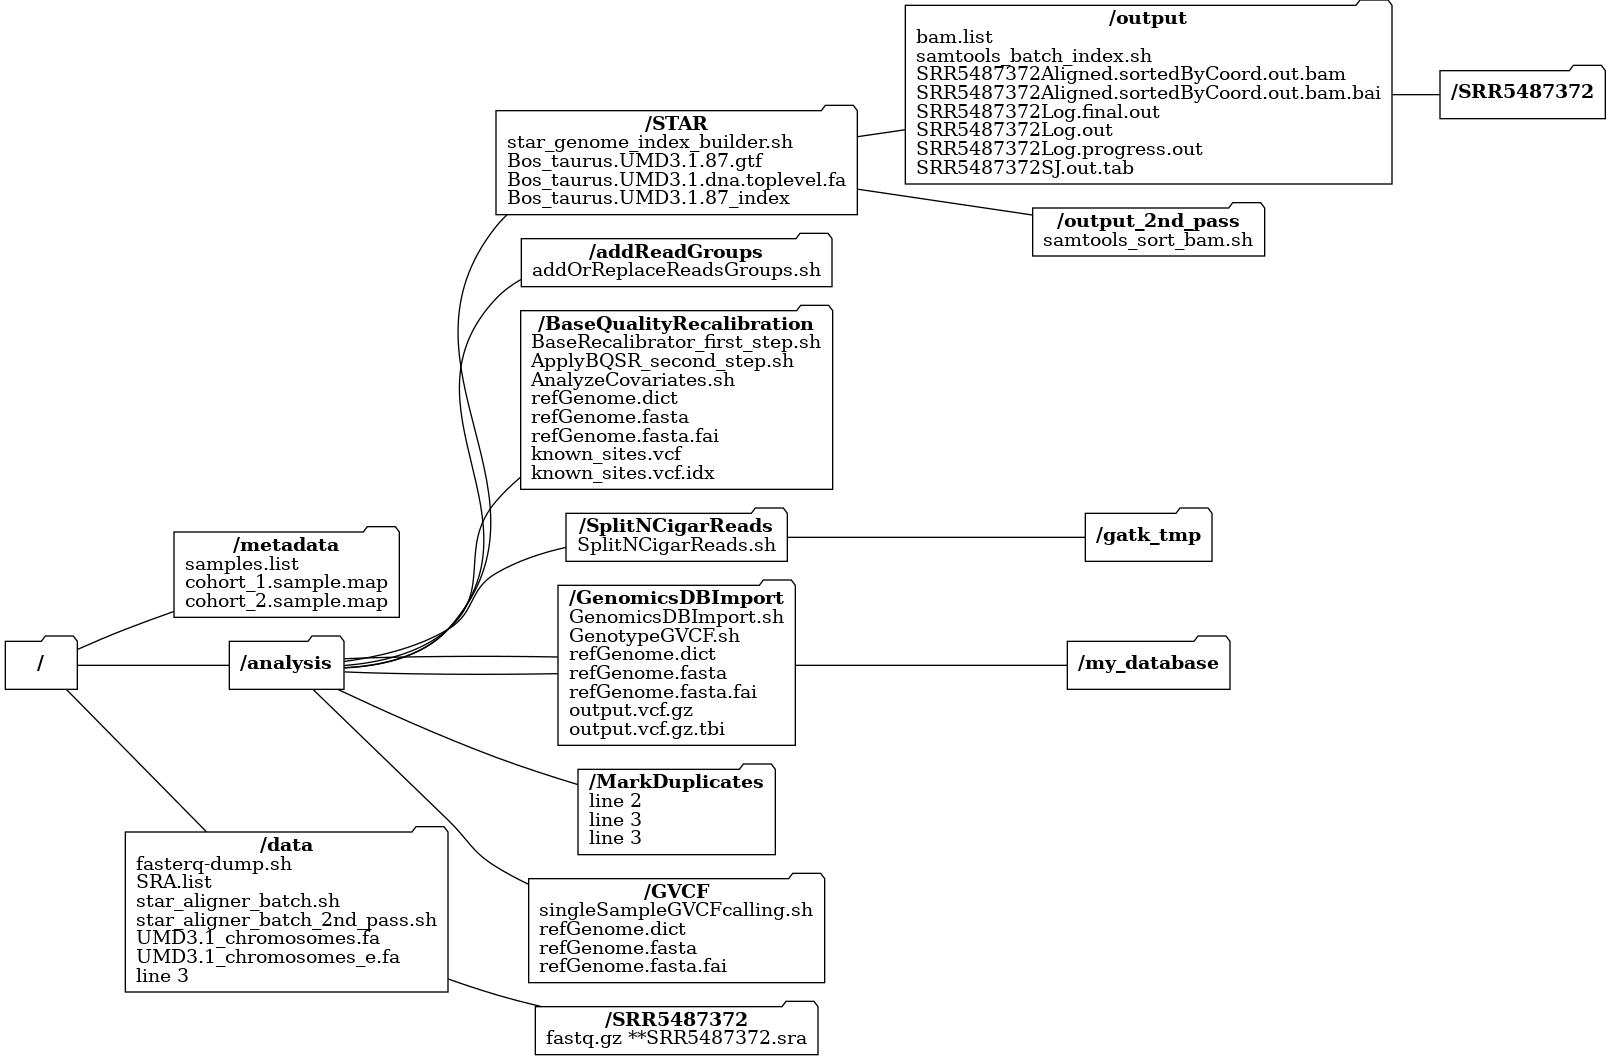
\includegraphics[width=\textwidth]{misc/tree.png}
\caption[caption] {long desc.}

\end{center}
\end{figure}





\subsection{Downloading raw sequences from NCBI SRA}

In this tutorial, we will use complete RNAseq datasets derived from primary macrophages of cows  in response to the infection by \textit{Mycobacterium avium ssp. paratuberculosis } (MAP), the etiological agent of paratuberculosis, or Johne’s disease (JD) \cite{Ariel2021}. However, rather than using the 72 samples presented in the article, we will use a subset of 24 representative samples. The \textbf{SRA.list} file located in the data folder contains the SRA identifiers of these 24 samples:

\begin{verbatim}
SRS2153774
SRS2153779
SRS2153781
...
SRS2153841
SRS2153845
\end{verbatim}


To download these sequences (X Gb), navigate to the /data directory and download the 24 samples with the prefetch command from the SRAtoolkit:

\begin{verbatim}
prefetch --option-file SRA.list
\end{verbatim}

To extract fastq files from .sra files, the fasterq-dump command is required. For example, the following command will produce SRR5487396\_R1.fastq.gz and SRR5487396\_R2.fastq.gz files from the SRR5487396 .sra archive.

\begin{verbatim}
fasterq-dump --split-files SRR5487396/SRR5487396.sra
\end{verbatim}

In practice, you will want to extract all downloaded sequence read archives, which are nested in distinct folders. Navigate to the /data folder and use the following qsub command to lauch the faster-qdump commands sequentially:

\begin{verbatim}
qsub -V -S /bin/bash -cwd -j y -pe smp 12 faster-qdump_sequential.sh
\end{verbatim}

where faster-qdump\_sequential.sh is a bash script containing instructions for the SGE workload manager and the code to iterate on all downloaded sequence read archives and to produce the forward and reverse fastq files.

\begin{verbatim}
#! /bin/bash
#$ -N 'fasterq-dump'
#$ -o ./faster-qdump_log.txt
	
for i in `ls -d SRR*`; do
cd $i
fasterq-dump --split-files $i.sra
cd ..
done
\end{verbatim}


However, executing the latter script would take a lot of times. To take advantage of the parallel computing capacity of compute servers, one may consider launching SGE array jobs (tasks in parallel). To learn more about this, one can consult man pages from from SGE available eslewhere.

Before using the faster-qdump\_parallel.sh, we need to create a simple list file of the 24 SRR* folders present in the /data folder:

\begin{verbatim}
ls -d1 SRR5487???>SRR.list
\end{verbatim}

Be sure that the SRR.list file contains the 24 SRR identifiers (without the .sra extension) on separates lines before lauching the parallel version of fasterq.dump.sh with:
\begin{verbatim}
qsub -V -S /bin/bash -cwd -j y -t 1-24 -pe smp 4 faster-qdump_parallel.sh
\end{verbatim}

\noindent faster-qdump\_parallel.sh:
\begin{verbatim}
#!/bin/bash
#$ -N fasterq-dump
#$ -o ./fasterq-dump.$TASK_ID.log
	
input=$(head -n $SGE_TASK_ID SRR.list | tail -n 1)
	
cd $input
fasterq-dump --split-files $input.sra
cd ..
\end{verbatim}


Figure x show how a computationnaly intense task, namely the decompressing of an .sra archive, can be run at the same time with similar input files. This can be done by using the SGE task array capabilities. Technically, the same script is run multiple times, with different values taken by the single environment variable \$SGE\_TASK\_ID. Since many bioinformatic tasks used in this tutorial are computationally intensive, most of the scripts presented thereafter will be base on this model.










